\documentclass[tikz,border=3pt]{standalone}
\usetikzlibrary{arrows.meta,positioning,fit,backgrounds,shapes.geometric}

\newcommand{\ImplGpu}{GPU-Based}

\begin{document}
\sffamily\footnotesize
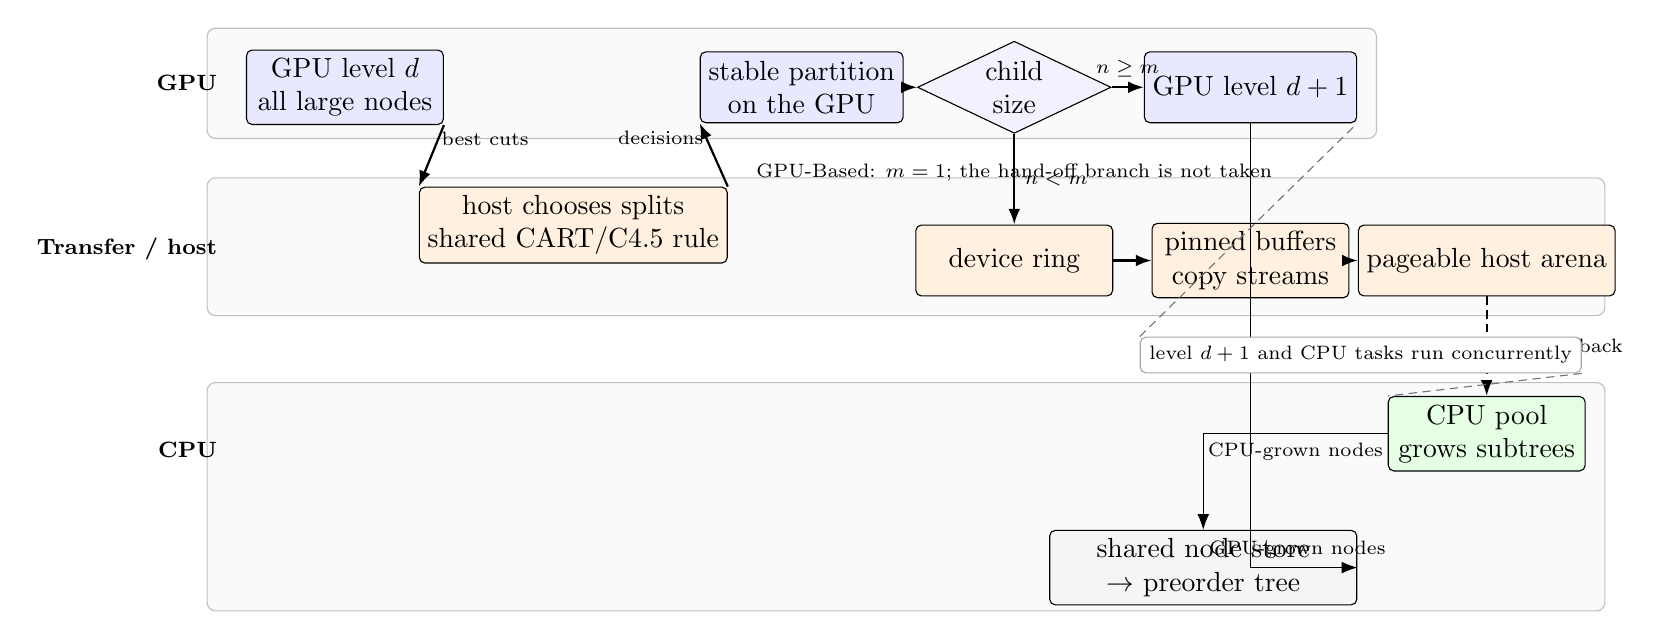
\begin{tikzpicture}[
  x=1cm,
  y=1cm,
  box/.style={
    draw,
    rounded corners=2pt,
    align=center,
    minimum height=9mm,
    minimum width=25mm,
    inner sep=3pt
  },
  gpu/.style={box, fill=blue!9},
  transfer/.style={box, fill=orange!12},
  cpu/.style={box, fill=green!10},
  decision/.style={
    diamond,
    draw,
    fill=blue!5,
    aspect=2.1,
    align=center,
    inner sep=1.5pt
  },
  flow/.style={-{Latex[length=2mm]}, thick},
  control/.style={-{Latex[length=2mm]}, densely dashed, thick},
  result/.style={-{Latex[length=2mm]}, thin},
  lane/.style={draw=black!25, fill=black!2, rounded corners=3pt},
  laneLabel/.style={font=\bfseries\footnotesize, anchor=east},
  note/.style={font=\scriptsize, align=center}
]

% Main boxes.
\node[gpu]      (level) at (0,2.4)
  {GPU level \(d\)\\all large nodes};
\node[transfer] (choose) at (2.9,0.65)
  {host chooses splits\\shared CART/C4.5 rule};
\node[gpu]      (partition) at (5.8,2.4)
  {stable partition\\on the GPU};
\node[decision] (size) at (8.5,2.4)
  {child\\size};
\node[gpu]      (next) at (11.5,2.4)
  {GPU level \(d+1\)};

\node[transfer] (ring) at (8.5,0.2)
  {device ring};
\node[transfer] (pinned) at (11.5,0.2)
  {pinned buffers\\copy streams};
\node[transfer] (arena) at (14.5,0.2)
  {pageable host arena};
\node[cpu]      (tasks) at (14.5,-2.0)
  {CPU pool\\grows subtrees};
\node[box, fill=black!4, minimum width=39mm] (store) at (10.9,-3.7)
  {shared node store\\\(\rightarrow\) preorder tree};

% Lane backgrounds.
\begin{scope}[on background layer]
  \node[lane, fit={(-1.75,3.15) (13.1,1.75)}, inner sep=0] (gpuLane) {};
  \node[lane, fit={(-1.75,1.25) (16.0,-0.5)}, inner sep=0] (hostLane) {};
  \node[lane, fit={(-1.75,-1.35) (16.0,-4.25)}, inner sep=0] (cpuLane) {};
\end{scope}
\node[laneLabel] at (-1.5,2.45) {GPU};
\node[laneLabel] at (-1.5,0.35) {Transfer / host};
\node[laneLabel] at (-1.5,-2.2) {CPU};

% Current GPU level and host split decision.
\draw[flow] (level.south east) -- node[above right,note] {best cuts} (choose.north west);
\draw[flow] (choose.north east) -- node[above left,note] {decisions} (partition.south west);
\draw[flow] (partition) -- (size);

% Size-based branch.
\draw[flow] (size) -- node[above,note] {\(n\ge m\)} (next);
\draw[flow] (size.south) -- node[right,note] {\(n<m\)} (ring.north);

% Asynchronous hand-off.
\draw[flow] (ring) -- (pinned);
\draw[flow] (pinned) -- (arena);
\draw[control] (arena) -- node[right,note] {host callback} (tasks);

% Both concurrent paths contribute to one tree.
\draw[result] (next.south) |- node[pos=.72,above,note] {GPU-grown nodes} (store.east);
\draw[result] (tasks.west) -| node[pos=.25,below,note] {CPU-grown nodes} (store.north);

% Explicit overlap cue and GPU-only note.
\node[note, draw=black!35, rounded corners=2pt, fill=white]
  (overlap) at (12.9,-1.0)
  {level \(d+1\) and CPU tasks run concurrently};
\draw[densely dashed, black!55] (overlap.north west) -- (next.south east);
\draw[densely dashed, black!55] (overlap.south east) -- (tasks.north west);

\node[note, anchor=north] at (8.5,1.55)
  {\ImplGpu{}: \(m=1\); the hand-off branch is not taken};

\end{tikzpicture}
\end{document}
